\setcounter{page}{84}
\setcounter{figure}{0}
\setcounter{chapter}{9}

\raggedright 

\chapter{Fuerzas variables, potencia, fuerza y energia potencial }
\label{cap:cap10}
\vspace{-15ex}

\raggedright
En general hemos estudiado situaciones donde las fuerzas se consideran constantes. Sin embargo, en muchos fenómenos reales, las fuerzas cambian de valor dependiendo de la posición o el tiempo. A estas fuerzas les llamamos \textbf{fuerzas variables}, y su análisis requiere herramientas más precisas, como el uso del cálculo o métodos gráficos. \\[.35cm]

Por otro lado, entender solo la fuerza o el trabajo no basta para describir completamente los procesos físicos: también es importante saber qué tan rápido se realiza ese trabajo. Esta idea nos lleva al concepto de \textbf{potencia}, que mide la cantidad de energía transferida o transformada por unidad de tiempo.


\tikzstyle{startstop} = [rectangle, rounded corners, minimum width=3cm, minimum height=1cm,text centered, draw=black, fill=blue!15]
\tikzstyle{process} = [rectangle, rounded corners, minimum width=3cm, minimum height=1cm, text centered, draw=black, fill=green!15]
\tikzstyle{arrow} = [thick,->,>=stealth]

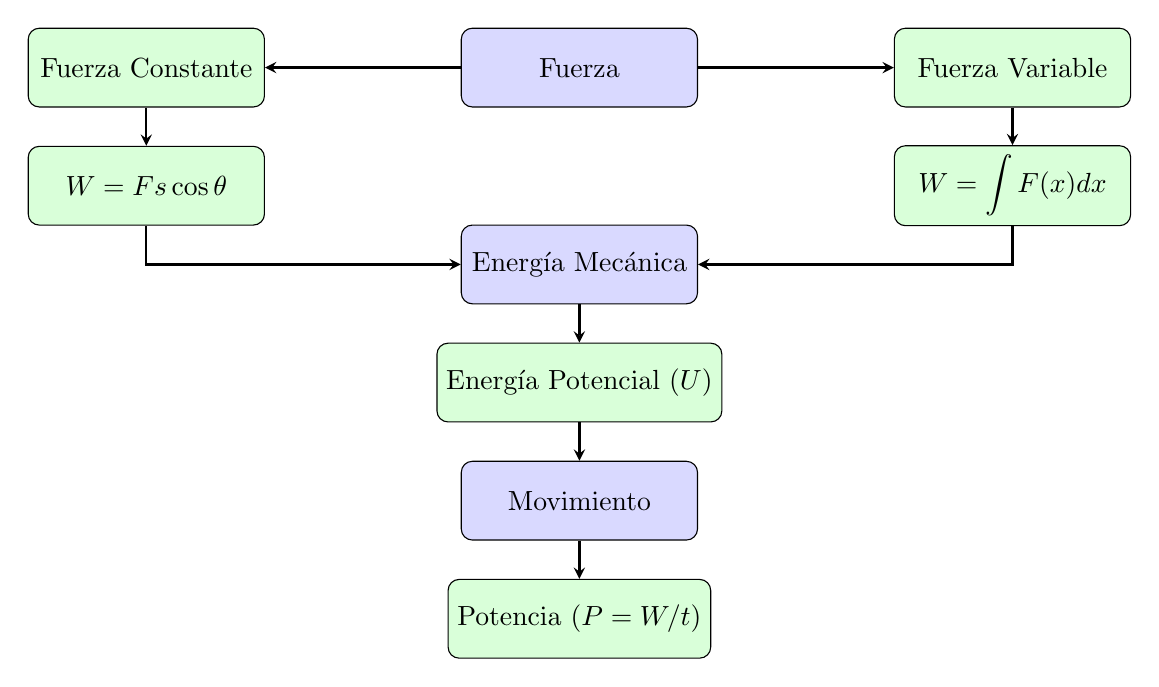
\begin{tikzpicture}[node distance=1.5cm]

% Nodes
\node (force) [startstop] {Fuerza};
\node (constant) [process, left of=force, xshift=-4cm] {Fuerza Constante};
\node (variable) [process, right of=force, xshift=4cm] {Fuerza Variable};
\node (work1) [process, below of=constant] {$W = Fs\cos\theta$};
\node (work2) [process, below of=variable] {$W = \displaystyle \int F(x)dx$};
\node (mechanical) [startstop, below of=force, yshift=-1cm] {Energía Mecánica};
\node (potential) [process, below of=mechanical] {Energía Potencial ($U$)};
\node (motion) [startstop, below of=potential] {Movimiento};
\node (power) [process, below of=motion] {Potencia ($P = W/t$)};

% Arrows
\draw [arrow] (force) -- (constant);
\draw [arrow] (force) -- (variable);
\draw [arrow] (constant) -- (work1);
\draw [arrow] (variable) -- (work2);
\draw [arrow] (work1.south) |- (mechanical.west);
\draw [arrow] (work2.south) |- (mechanical.east);
\draw [arrow] (mechanical) -- (potential);
\draw [arrow] (potential) -- (motion);
\draw [arrow] (motion) -- (power);

\end{tikzpicture}


\section{Fuerzas variables}

El \textbf{trabajo realizado por fuerzas variables} es un concepto fundamental en la física, especialmente cuando se analiza la mecánica de cuerpos que están sometidos a fuerzas que no permanecen constantes a lo largo de su desplazamiento. A diferencia del trabajo realizado por fuerzas constantes, donde la relación entre la fuerza y el desplazamiento es directa y simple, en el caso de fuerzas variables la situación se complica, ya que la magnitud y la dirección de la fuerza cambian en cada punto del trayecto. \\[.35cm]

Para abordar este tipo de problemas, se recurre a \textbf{la integración}, ya que el trabajo realizado por una fuerza variable a lo largo de un trayecto es igual a la integral de la fuerza a lo largo de la distancia recorrida. Matemáticamente, el trabajo \( W \) realizado por una fuerza \( F(x) \) que depende de la posición \( x \) se expresa como

\begin{equation}
W = \int_{x_1}^{x_2} F(x) \, dx
\end{equation}

donde \( F(x) \) es la fuerza en función de la posición, y \( x_1 \) y \( x_2 \) son los límites de la posición del objeto. \\[.35cm]

En este contexto, el \textbf{análisis gráfico} es una herramienta poderosa para comprender la relación entre la fuerza y la posición. Si se representa gráficamente la fuerza \( F(x) \) en función de la posición \( x \), el área bajo la curva de esa gráfica entre dos puntos \( x_1 \) y \( x_2 \) nos proporciona el trabajo realizado (ver Figura \ref{fig:W_F_x}). Este enfoque visual permite identificar claramente cómo la fuerza varía a lo largo del trayecto y facilita la interpretación de los resultados. \\[.35cm]

\begin{figure}[h!]
    \centering
    \includegraphics[width=300px]{planeamiento_didactico/figuras/area_bajo_curva_W.pdf}
    \caption{El \'area bajo la curva en una gr\'afica de fuerza en funci\'on de la posici\'on representa el trabajo que realiza dicha fuerza.}
    \label{fig:W_F_x}
\end{figure}

\section{Potencia}
La \textbf{potencia} es una magnitud física que mide la rapidez con la que se realiza un trabajo o se transfiere energía. En términos generales, mientras el trabajo nos indica cuánta energía se transfiere, la potencia nos dice \textbf{qué tan rápido} ocurre esa transferencia. Este concepto resulta especialmente importante en ingeniería, donde la eficiencia y el desempeño de sistemas mecánicos, eléctricos y térmicos dependen de la tasa de trabajo que pueden realizar. \\[.35cm]

La \textbf{potencia media} (\( P_{\text{med}} \)) es  el trabajo medio efectuado por unidad de tiempo

\begin{equation}
P_{\text{prom}} = \frac{\Delta W}{\Delta t}
\end{equation}

donde \( \Delta W \) es el trabajo realizado y \( \Delta t \) es el intervalo de tiempo en el cual se realiza ese trabajo. \\[.35cm]

Sin embargo, en muchos casos es importante analizar la \textbf{potencia instantánea}, que describe la potencia en un momento específico. Matemáticamente, la potencia instantánea \( P \) se define como

\begin{equation}
P = \frac{dW}{dt}
\end{equation}

En situaciones donde una fuerza \( \vec{F} \) actúa sobre un objeto que se mueve con una velocidad \( \vec{v} \), la potencia instantánea también puede expresarse como el producto escalar:

\begin{equation}
P = \vec{F} \cdot \vec{v}=Fv\cos\theta
\end{equation}

Esto refleja que la potencia depende tanto de la magnitud de la fuerza como de su orientación relativa a la velocidad: solo la componente de la fuerza en la dirección del movimiento contribuye al trabajo, y por ende, a la potencia. \\[.35cm]

La potencia es crucial en el diseño y análisis de motores, generadores, sistemas de transmisión, y prácticamente cualquier dispositivo que implique la conversión o el uso de energía. Una alta potencia puede ser necesaria para mover grandes cargas, acelerar objetos en poco tiempo, o mantener sistemas industriales operando de manera eficiente.\\[.35cm]

En resumen, el concepto de potencia conecta el trabajo, el tiempo y el movimiento de una manera fundamental para comprender y optimizar el funcionamiento de sistemas físicos.\\[.35cm]


La unidad de potencia en el S.I es el \textit{watt} (W)
$$1\units{W}=1\units{J/s}. $$

\begin{table}[h!]
\caption{Algunas unidades de potencia}
\label{tab:W}
\centering
\begin{tabular}{lc}
\toprule
\textbf{Unidad}&\textbf{Equivalencia en W} \\[.35cm]
\toprule
\textit{kilovatio} (kW)& $1000$ \\[.35cm]
\textit{caballo de fuerza} (hp) & $\approx 746$ \\[.35cm]
\textit{caballo de vapor} (CV)& $\approx 735$\\[.35cm]
\toprule
\end{tabular}
\end{table}


\section{Fuerza y energía potencial}

En el estudio de los sistemas físicos, resulta fundamental comprender la relación entre fuerzas y energía. En particular, cuando una fuerza es de tipo conservativa, es posible asociarle una función de \textit{energía potencial} que describe cómo varía la energía almacenada en el sistema en función de la posición. \\[.35cm]

Formalmente, si $\vec{F}$ es una fuerza conservativa, existe una función escalar $U$ (la energía potencial) tal que:

\begin{equation}
F_{x} = -\frac{\partial U}{\partial x}, \qquad F_{y} = -\frac{\partial U}{\partial y}, \qquad F_{z} = -\frac{\partial U}{\partial z}.
\end{equation}

Estas relaciones expresan que la fuerza actúa en la dirección de mayor disminución de la energía potencial. Para simplificar la notación, la ecuación anterior puede escribirse de manera compacta como

\begin{equation}
\vec{F} = -\nabla U,
\end{equation}

donde $\nabla$ representa el \textit{operador diferencial nabla}. Este operador actúa sobre funciones escalares para producir un campo vectorial, y se define como

\begin{equation}
\nabla \Phi = \left( \frac{\partial \Phi}{\partial x}, \frac{\partial \Phi}{\partial y}, \frac{\partial \Phi}{\partial z} \right) = \frac{\partial \Phi}{\partial x}\, \hat{\iota} + \frac{\partial \Phi}{\partial y}\, \hat{\jmath} + \frac{\partial \Phi}{\partial z}\, \hat{\kappa},
\end{equation}

donde $\Phi(x,y,z)$ es una función escalar, y $\hat{\iota}, \hat{\jmath}, \hat{\kappa}$ son los vectores unitarios en las direcciones $x$, $y$, y $z$, respectivamente.\\[.35cm]

Esta formulación conecta elegantemente la noción de fuerza con la variación espacial de la energía potencial, y es fundamental para el análisis de sistemas conservativos en mecánica clásica y más allá.

\begin{wwteorema}{Energ\'ia potencial gravitacional y peso}
    Si consideramos $U_g=mgy$,
    $$\vec{F}_g=-\nabla(mgy)=-\displaystyle \left(\frac{\partial (mgy)}{\partial x}\hat{\iota}+\frac{\partial (mgy)}{\partial y}\hat{\jmath}+\frac{\partial (mgy)}{\partial z}\hat{\kappa} \right)=-mg\hat{\jmath}$$
\end{wwteorema}




